\documentclass{article} % Defines the document class, article is commonly used
\usepackage[shortlabels]{enumitem}
\usepackage{amsmath}    % Allows for more advanced math formatting
\usepackage{amssymb}    % Provides additional mathematical symbols
\usepackage{amsthm}     % \qed
\usepackage{graphicx}   % image
\usepackage{float}      % image placement
\usepackage{hyperref}
\hypersetup{
    colorlinks=true,       % false: boxed links; true: colored links
    linkcolor=black,       % color of internal links
}
\usepackage[margin=1.5in]{geometry}

\begin{document}

\title{EEC133 Lab 1 Report}
\author{Josias Moreno Ixta, Michael Chen, Tao Wang, Xaviera Azodoh}
\date{\today}

\maketitle
\tableofcontents
\pagebreak

\section*{Part 1 Antenna Construction}
\addcontentsline{toc}{section}{Part 1 Antenna Construction}
\begin{figure}[H]
    \centering
    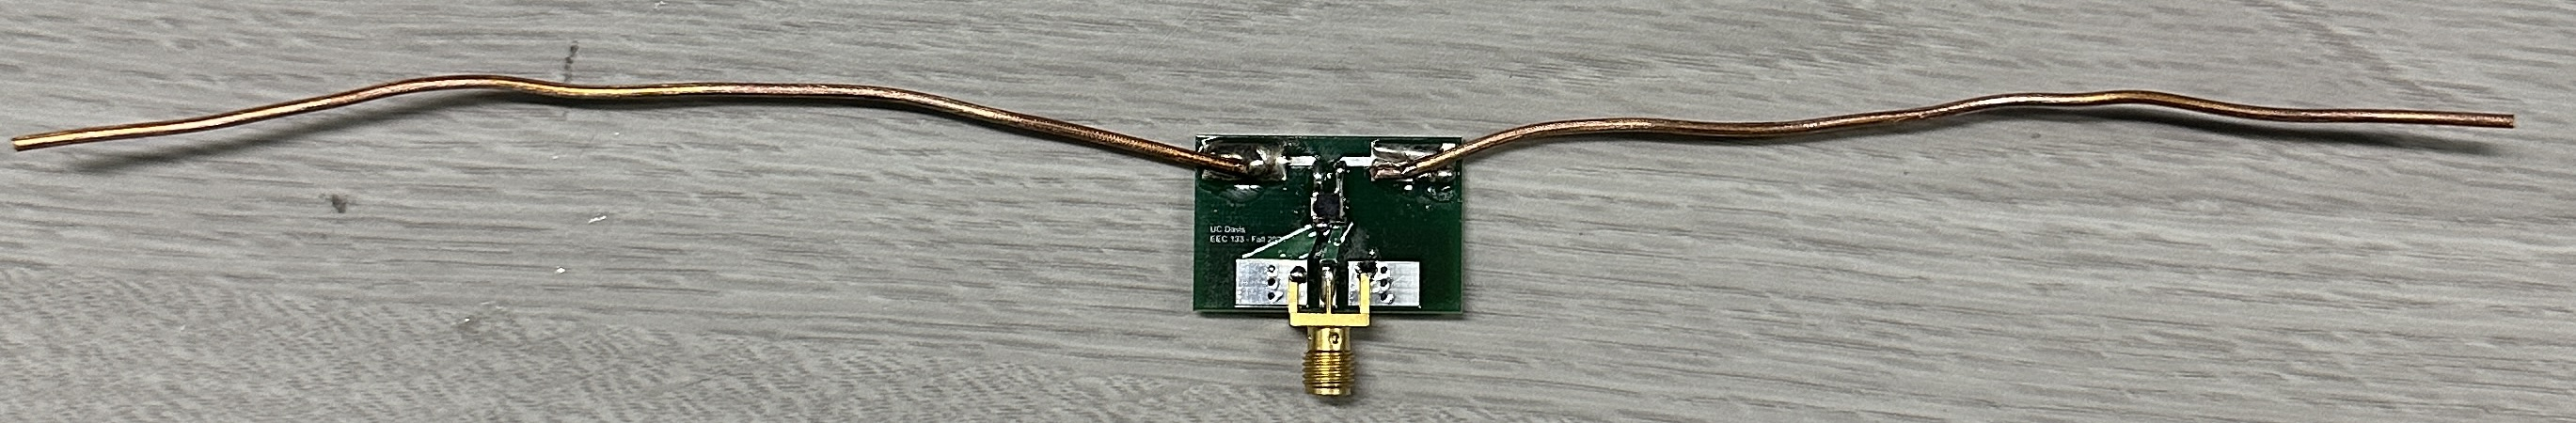
\includegraphics[width=1\textwidth]{./image/figure1.jpeg}
    \caption{Dipole Antenna}
\end{figure}

\section*{Part 2 Basic VNA Measurements}
\addcontentsline{toc}{section}{Part 2 Basic VNA Measurements}

\subsection*{Step 1}
\addcontentsline{toc}{subsection}{Step 1}
\begin{figure}[H]
    \centering
    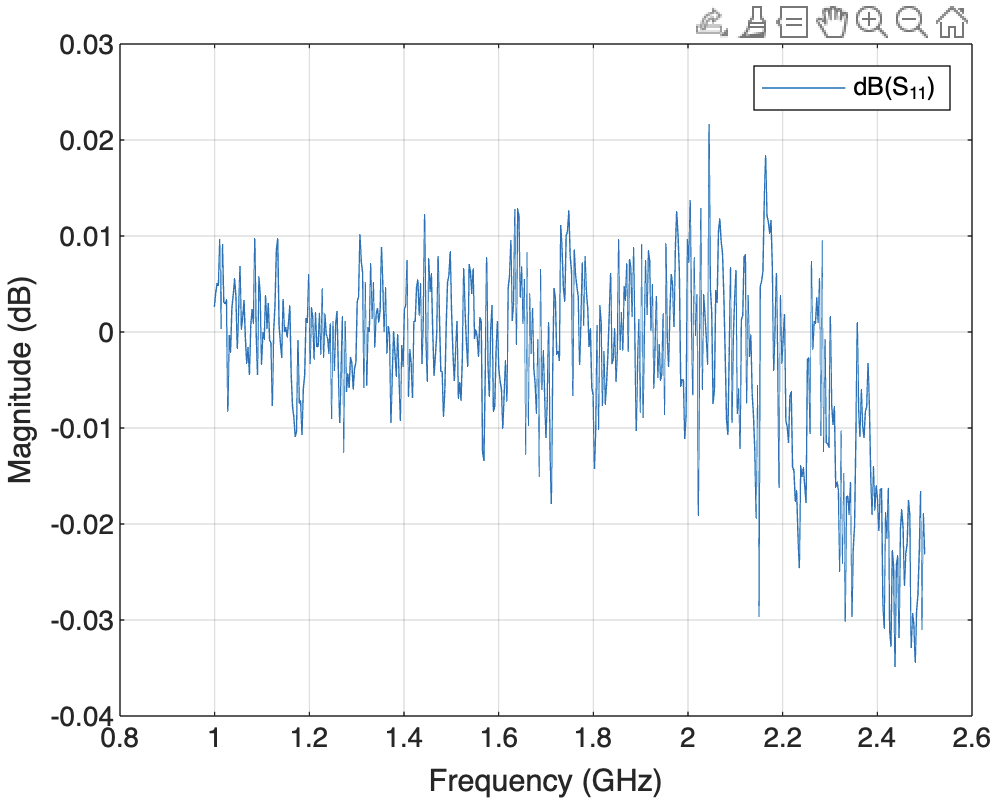
\includegraphics[width=0.5\textwidth]{./image/figure2.png}
    \caption{$S_{11}$ of Unterminated Cable}
\end{figure}

\begin{figure}[H]
    \centering
    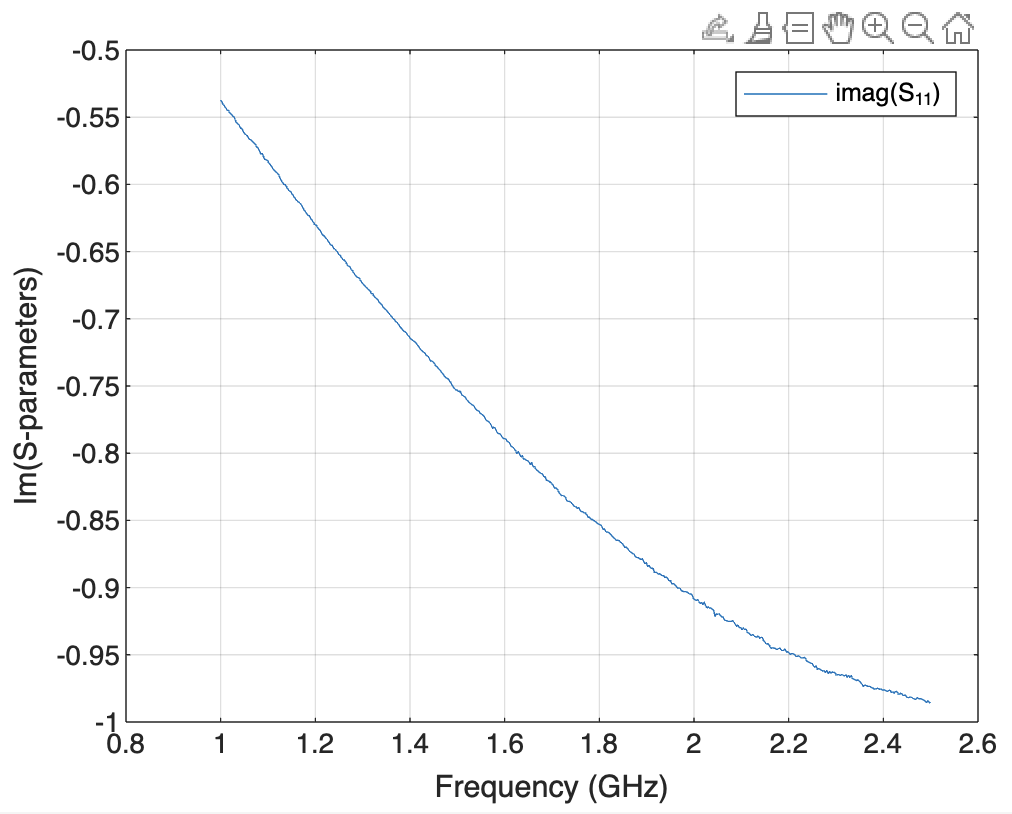
\includegraphics[width=0.5\textwidth]{./image/figure3.png}
    \caption{Imaginary $S_{11}$ of Unterminated Cable}
\end{figure}

\subsection*{Step 2}
\addcontentsline{toc}{subsection}{Step 2}

Cable Length: 25 inches long

\subsubsection*{Short Circuit S-Parameter}
\addcontentsline{toc}{subsubsection}{Short Circuit S-Parameter}
\begin{figure}[H]
    \centering
    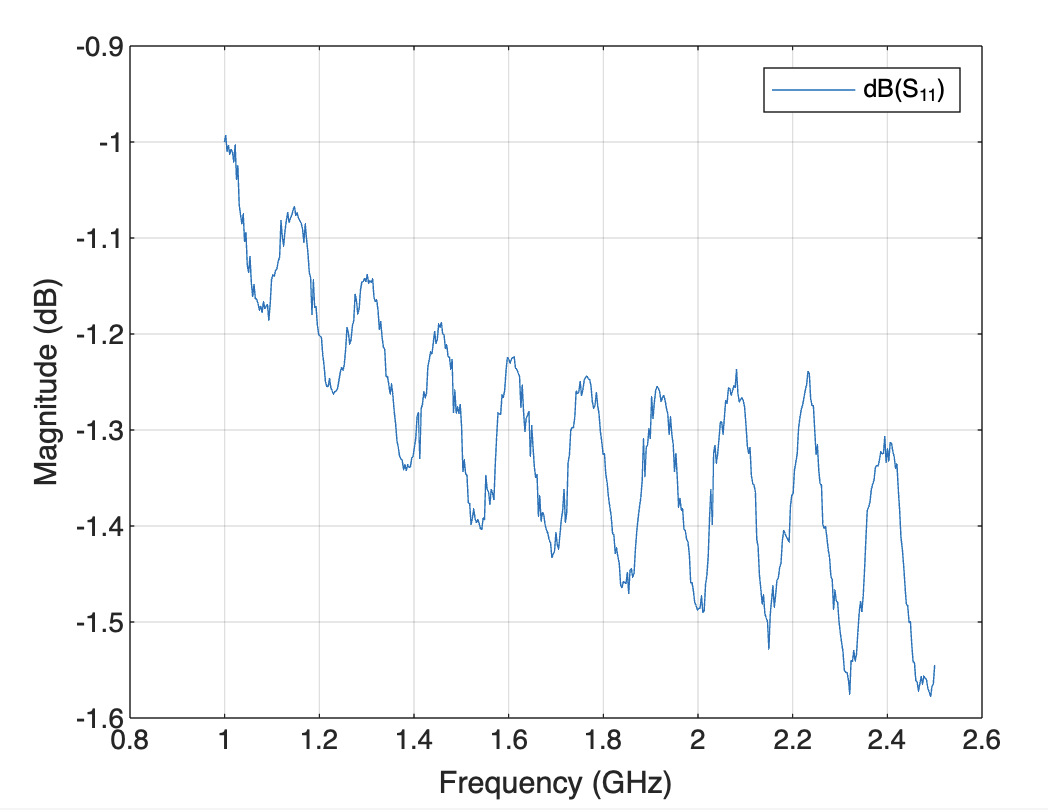
\includegraphics[width=0.5\textwidth]{./image/figure4.png}
    \caption{$S_{11}$ in a Short Circuit Transmission Line}
\end{figure}
\begin{figure}[H]
    \centering
    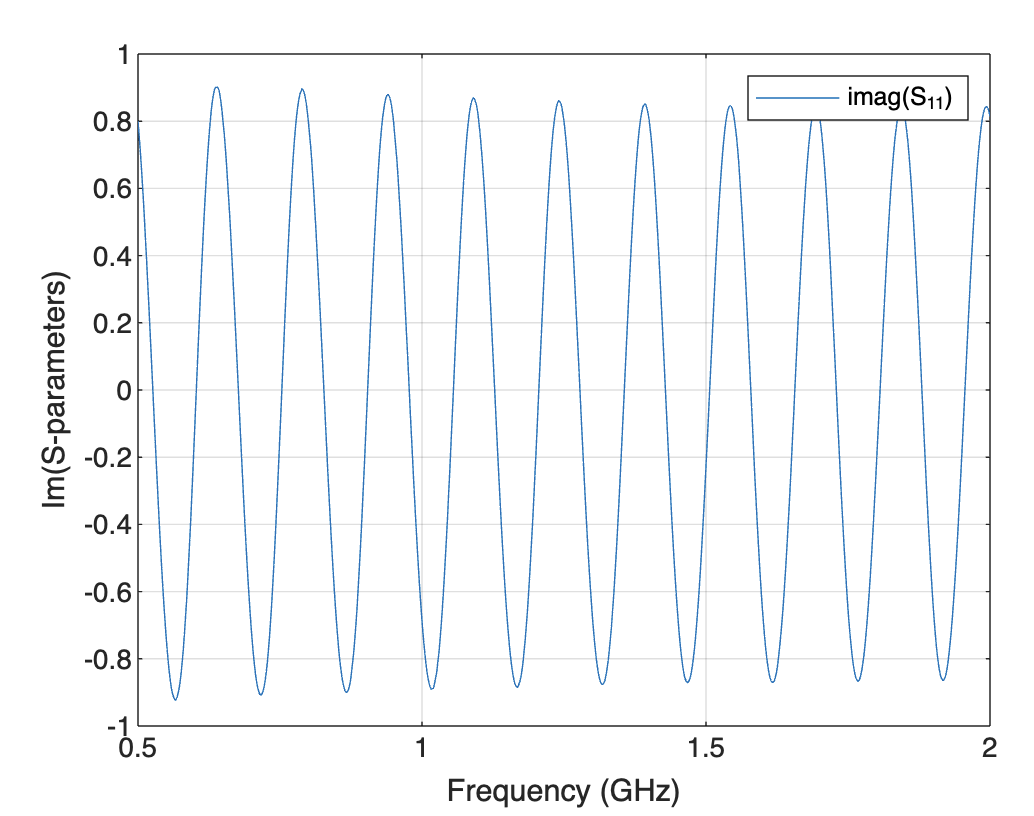
\includegraphics[width=0.5\textwidth]{./image/figure5.png}
    \caption{Reactance of $S_{11}$ in a Short Circuit Transmission Line}
\end{figure}

\subsubsection*{Open Circuit S-Parameter}
\addcontentsline{toc}{subsubsection}{Open Circuit S-Parameter}
\begin{figure}[H]
    \centering
    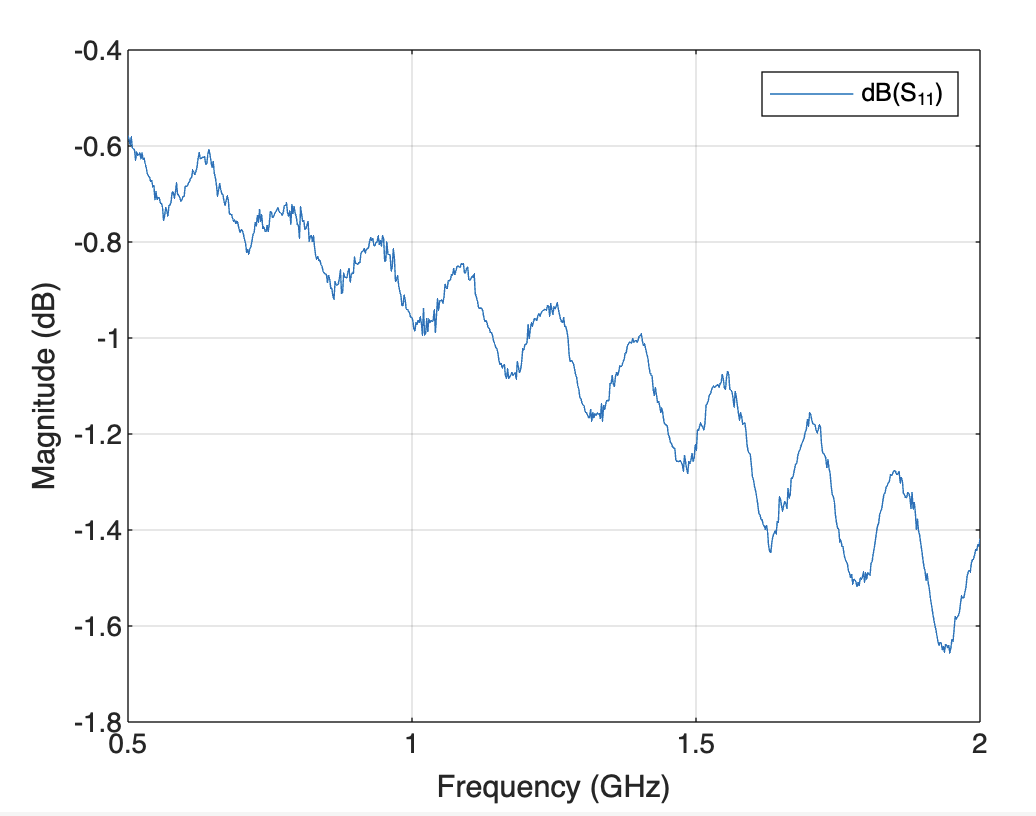
\includegraphics[width=0.5\textwidth]{./image/figure6.png}
    \caption{$S_{11}$ in a Open Circuit Transmission Line}
\end{figure}
\begin{figure}[H]
    \centering
    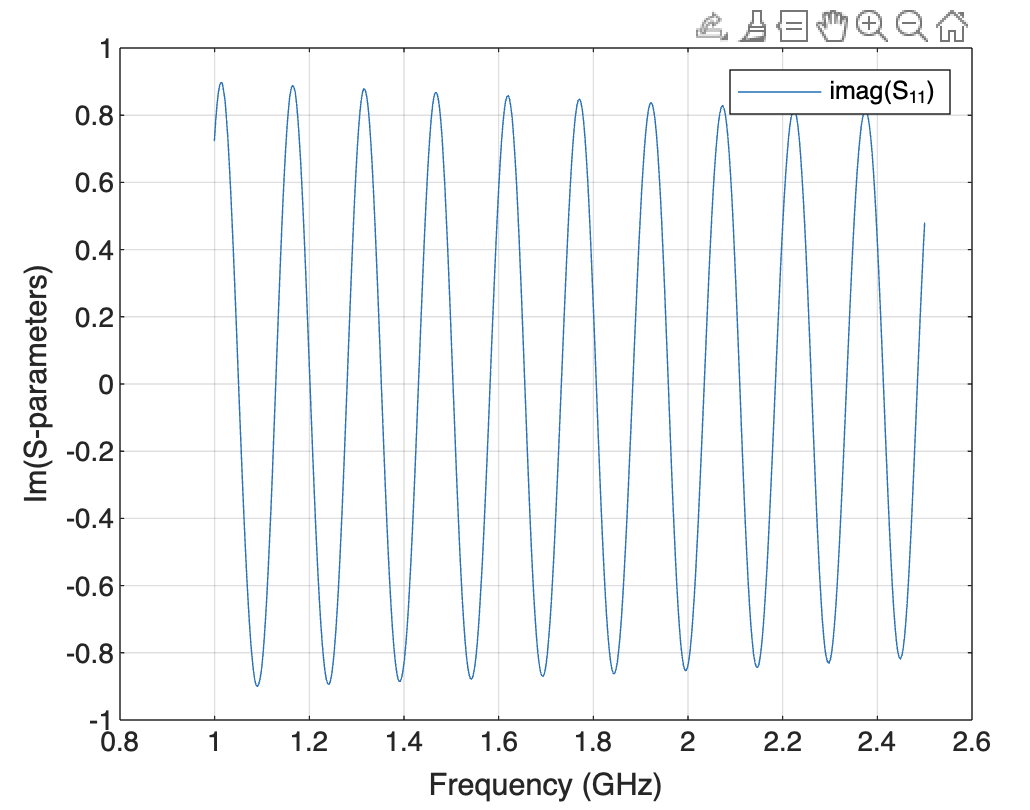
\includegraphics[width=0.5\textwidth]{./image/figure7.png}
    \caption{Reactance of $S_{11}$ in a Open Circuit Transmission Line}
\end{figure}

\subsubsection*{$50 \Omega$ Load Transmission Line S-Parameter}
\addcontentsline{toc}{subsubsection}{$50 \Omega$ Load Circuit S-Parameter}
\begin{figure}[H]
    \centering
    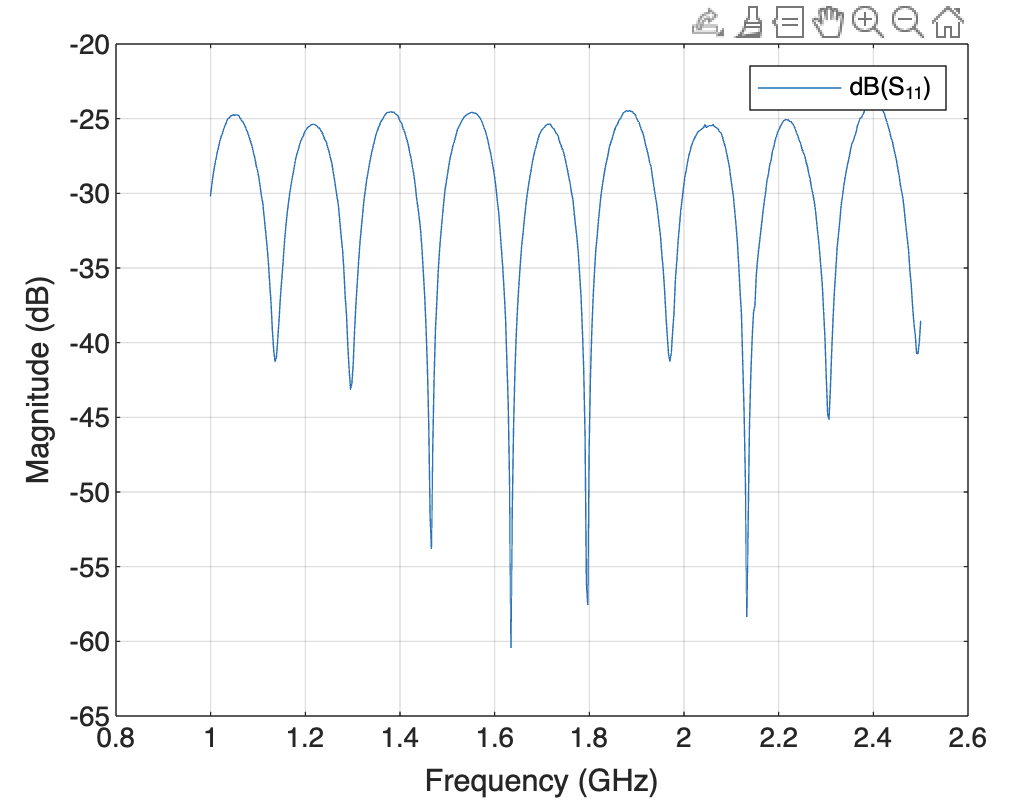
\includegraphics[width=0.5\textwidth]{./image/figure8.png}
    \caption{$S_{11}$ in a $50 \Omega$ Load Transmission Line}
\end{figure}
\begin{figure}[H]
    \centering
    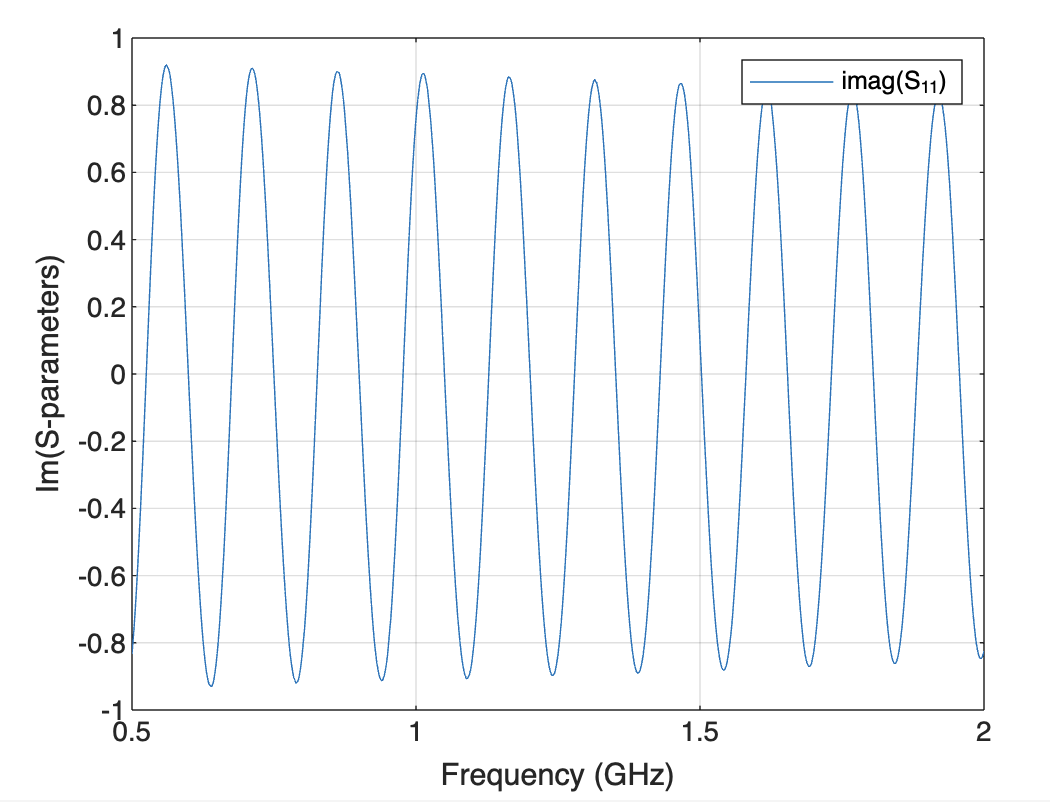
\includegraphics[width=0.5\textwidth]{./image/figure9.png}
    \caption{Reactance of $S_{11}$ in a $50 \Omega$ Load Circuit Transmission Line}
\end{figure}

\section*{Part 3 Antenna Measurements}
\addcontentsline{toc}{section}{Part 3 Antenna Measurements}
\subsection*{Step 1}
\addcontentsline{toc}{subsection}{Step 1}
\begin{figure}[H]
    \centering
    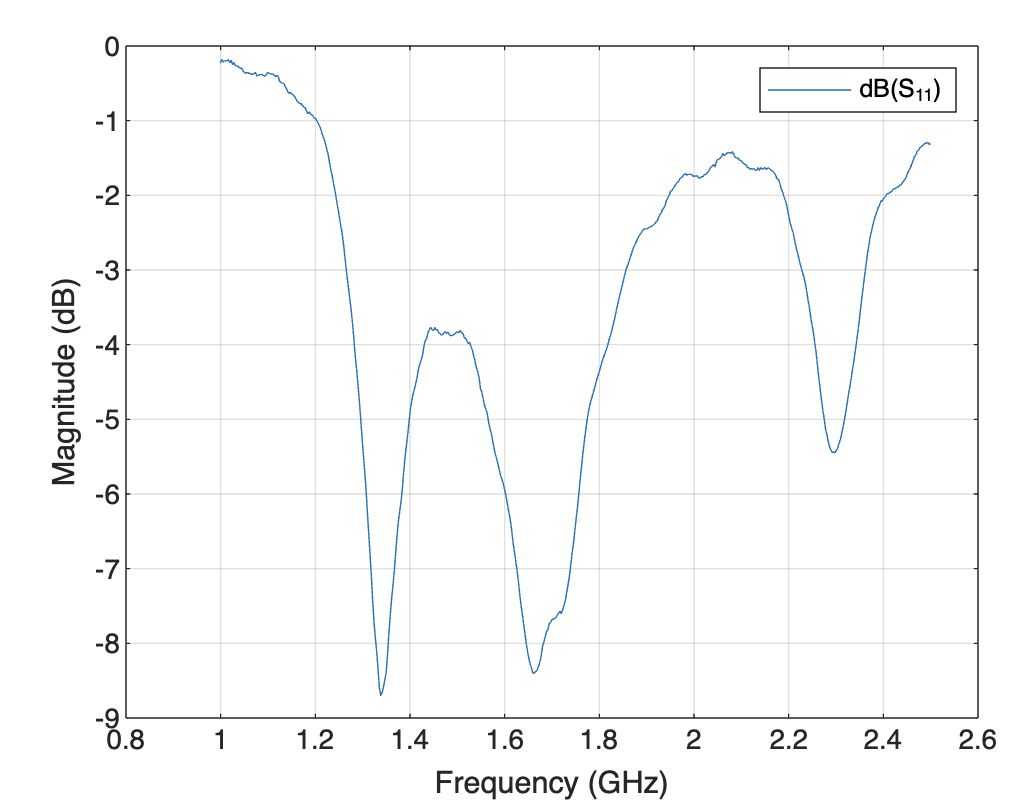
\includegraphics[width=0.5\textwidth]{./image/figure10.png}
    \caption{Dipole Antenna's $S_{11}$ Magnitude}
\end{figure}
\begin{figure}[H]
    \centering
    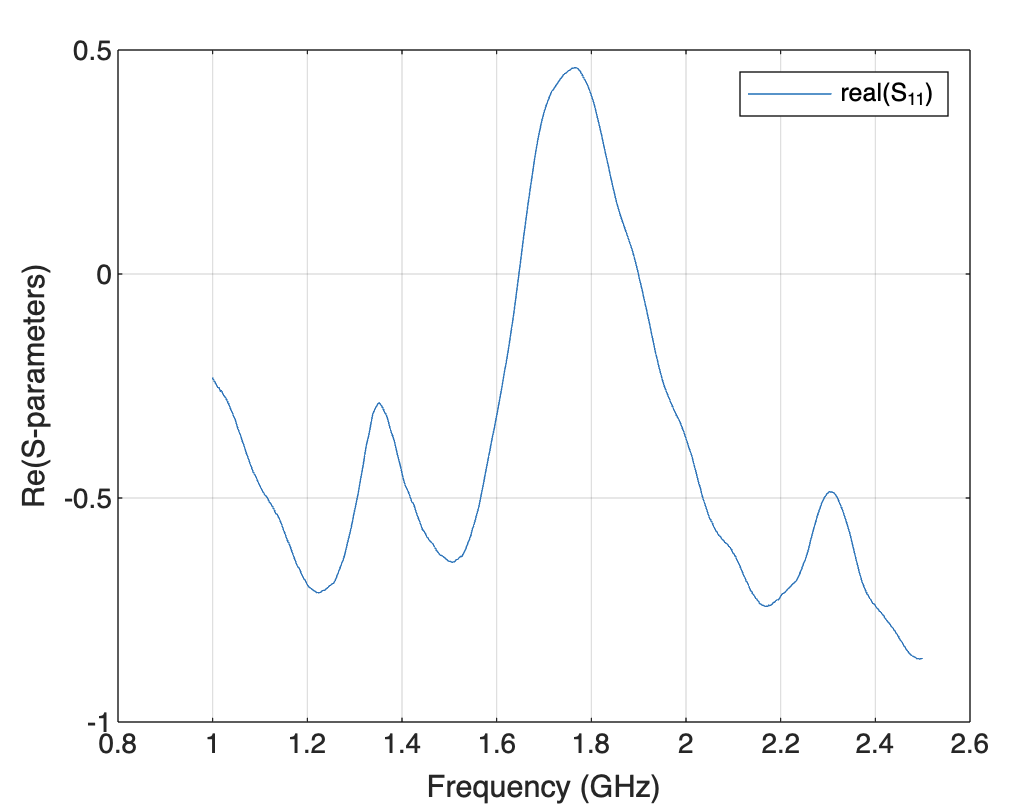
\includegraphics[width=0.5\textwidth]{./image/figure11.png}
    \caption{Dipole Antenna's Real Part of $S_{11}$}
\end{figure}
\begin{figure}[H]
    \centering
    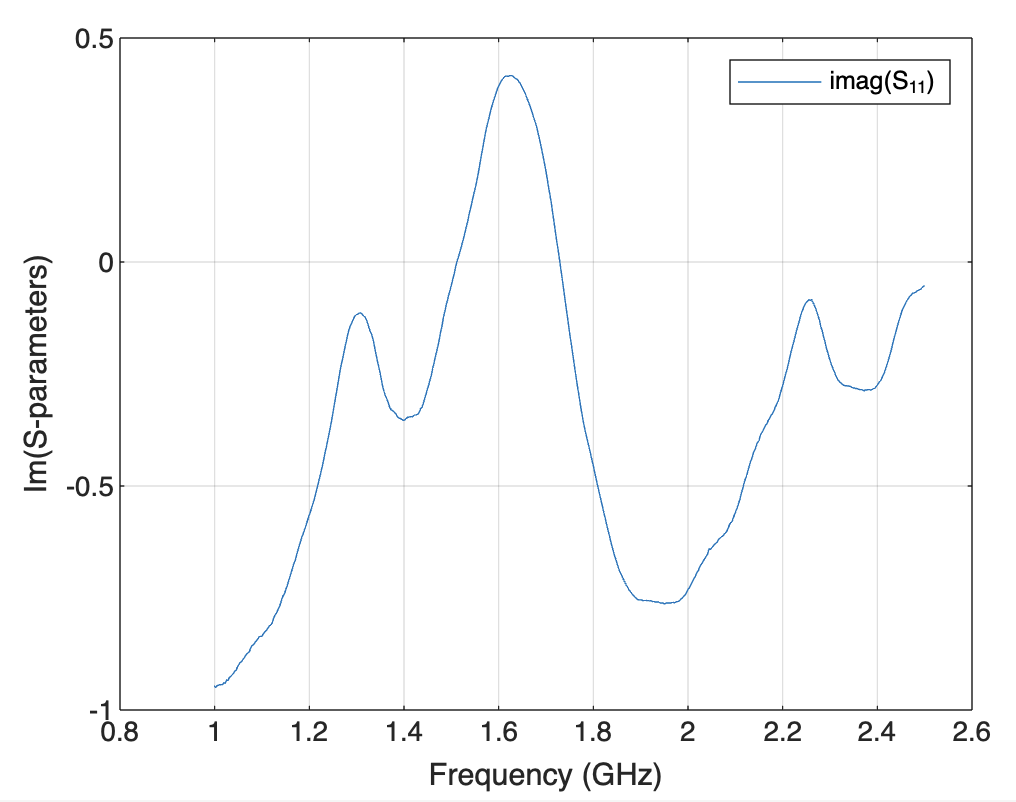
\includegraphics[width=0.5\textwidth]{./image/figure12.png}
    \caption{Dipole Antenna's Imaginary Part of $S_{11}$}
\end{figure}

\subsection*{Step 2}
\addcontentsline{toc}{subsection}{Step 2}
Distance between the two antennas: 10 feet.

\subsection*{Step 3}
\addcontentsline{toc}{subsection}{Step 3}

\begin{table}[h!]
    \centering
    \begin{tabular}{|c|c|}
        \hline
        \textbf{Angle (degrees)} & \textbf{$S_{21}$ (dB)} \\
        \hline
        0                        & -48.0                  \\
        10                       & -53.0                  \\
        20                       & -50.0                  \\
        30                       & -54.8                  \\
        40                       & -53.0                  \\
        50                       & -45.0                  \\
        60                       & -45.04                 \\
        70                       & -48.0                  \\
        80                       & -54.0                  \\
        90                       & -64.0                  \\
        100                      & -55.0                  \\
        110                      & -47.0                  \\
        120                      & -44.0                  \\
        130                      & -44.0                  \\
        140                      & -44.6                  \\
        150                      & -45.6                  \\
        160                      & -48.0                  \\
        170                      & -50.0                  \\
        180                      & -56.0                  \\
        \hline
    \end{tabular}
    \caption{$S_{21}$ when Dipole Antenna Faces Different Angle}
\end{table}
\begin{figure}[H]
    \centering
    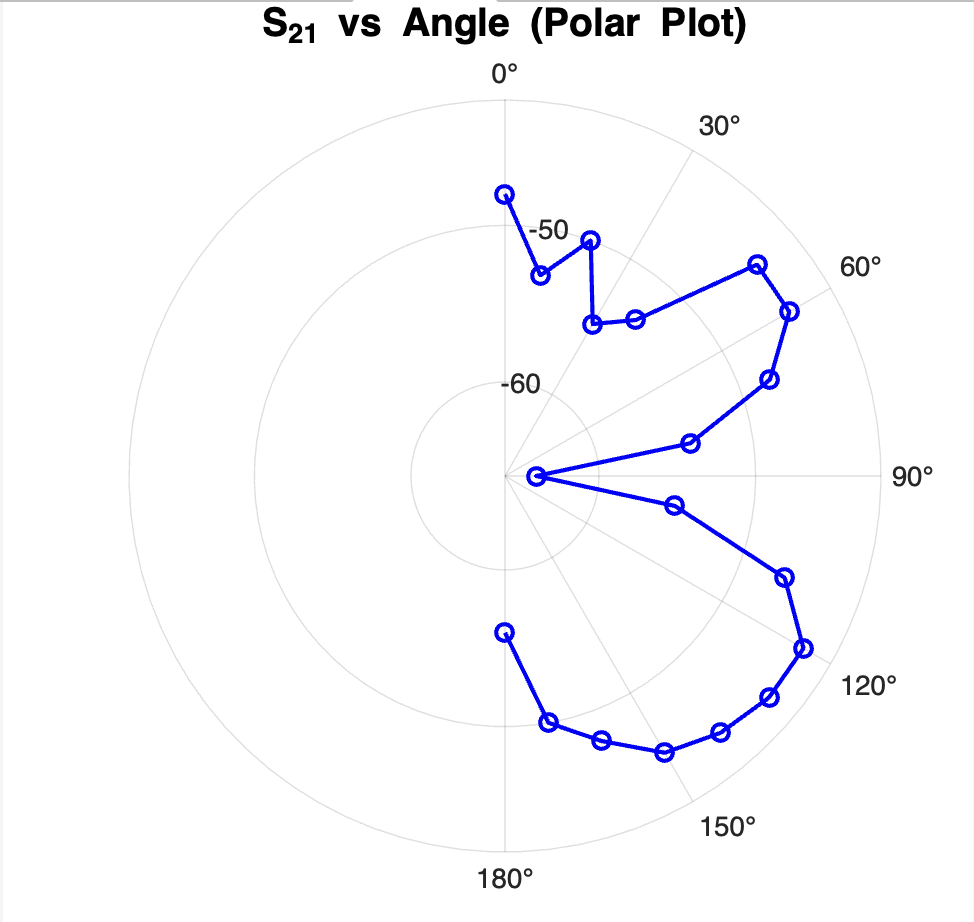
\includegraphics[width=0.5\textwidth]{./image/figure13.png}
    \caption{$S_{21}$ when Dipole Antenna Faces Different Angle}
\end{figure}

\subsection*{Step 4}
\addcontentsline{toc}{subsection}{Step 4}
$S_{21} = -64$ dB at $180 \deg$ and vertical to the floor.

\section*{Part 4 Post Lab Questions}
\addcontentsline{toc}{section}{Part 4 Post Lab Questions}
\subsection*{Q1}
\addcontentsline{toc}{subsection}{Q1}

\begin{enumerate}[label=(\alph*)]
    \item The measurement of the unterminated transmission line matches with the theory. The $S_{11}$ parameter is close to 0 dB, which means all input wave was reflected.
    \item See the plots from Figure 4 to Figure 9. We expect from the transmission line theory that the open and short terminal will reflect the wave entirely, but the $50 \Omega$ matched end will allow waves to transmit.

          The measurement result largely agrees with the theory. The short and open circuit transmission line has a larger $S_{11}$, which means most waves were reflected. Furthermore, their imaginary part of $S_{11}$ is out of phase by 180 degrees because their reflection coefficients are 1 and -1.

          The matched load measurement results also aligned with the theory. The $S_{11}$ was very small, which means most waves were transmitted.
\end{enumerate}

\subsection*{Q2}
\addcontentsline{toc}{subsection}{Q2}
The balun ensures a differential signal passes into two ends of the antenna. A signal with near-perfect opposite polarity is important for a dipole antenna because we assumed the signal is symmetrical.

\subsection*{Q3}
\addcontentsline{toc}{subsection}{Q3}
\begin{enumerate}
    \item We measured the dipole antenna to have a length of 0.3 meters.
    \item Since the PCB board has a relative permittivity of $\epsilon_r \approx 3.2$, the ratio between the dipole length and the wavelength is $\frac{l}{\lambda} = \frac{l \sqrt{\epsilon_r}}{\lambda_0}$, so we have the effective length as 0.54 meters.
\end{enumerate}

\subsection*{Q4}
\addcontentsline{toc}{subsection}{Q4}
See plots from Figure 10 to Figure 12 for the return loss. The following table shows the fraction of wavelength the dipole is at different resonant frequency
\begin{table}[h]
    \centering
    \begin{tabular}{|c|c|}
        \hline
        Frequency (GHz) & Fraction of Wavelength ($\frac{l}{\lambda}$) \\
        \hline
        1.34            & 2.41                                         \\
        1.66            & 2.99                                         \\
        2.29            & 4.12                                         \\
        \hline
    \end{tabular}
    \caption{Dipole Length Fraction at Different Frequency}
    \label{tab:yourlabel}
\end{table}

The result shows that the $S_{11}$ parameter is at the lowest when the dipole length is 1.34 times the wavelength. At this dipole length, the least amount of wave got reflected from the antenna.
The length, 0.54 m was used in the calculation because it accounts for the wavelength of the EM wave in different material. This is a more accurate approximation of the dipole length to wavelength ratio.

\subsection*{Q5}
\addcontentsline{toc}{subsection}{Q5}

We used the following formula to turn the real and imaginary part of the S parameter into the complex input impedance.

\[Z_{in} = Z_0 \left(\frac{1 + S_{11}}{1 - S_{11}}\right)\text{, where }Z_0 = 50 \Omega\]

\begin{figure}[H]
    \centering
    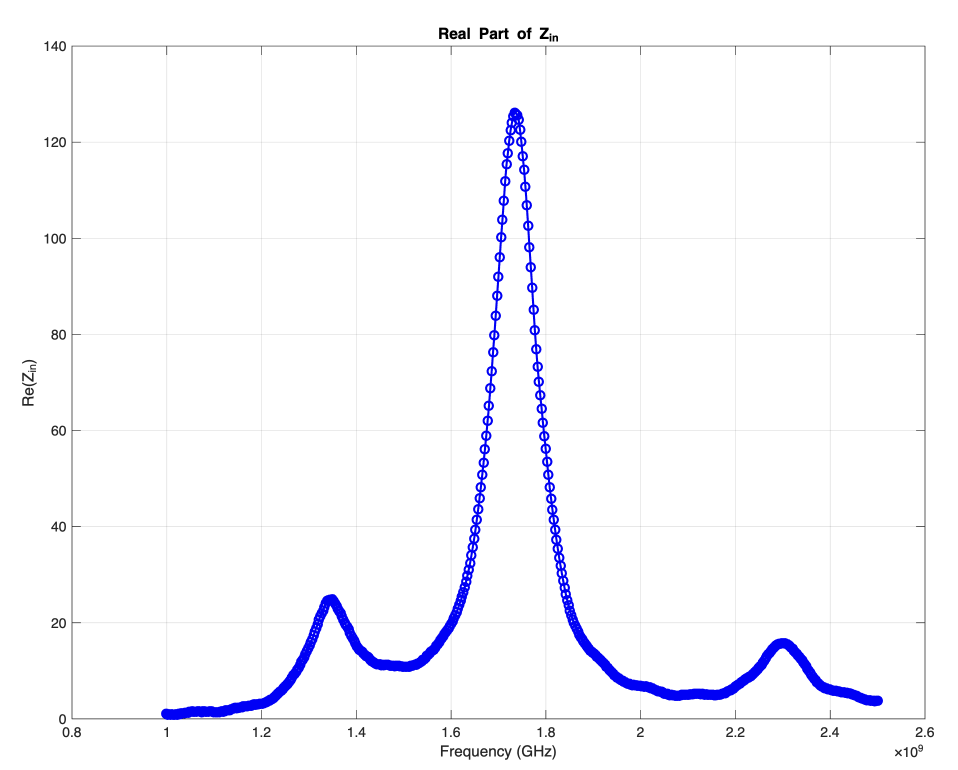
\includegraphics[width=0.5\textwidth]{./image/figure14.png}
    \caption{Real Part of Input Impedance}
\end{figure}

\begin{figure}[H]
    \centering
    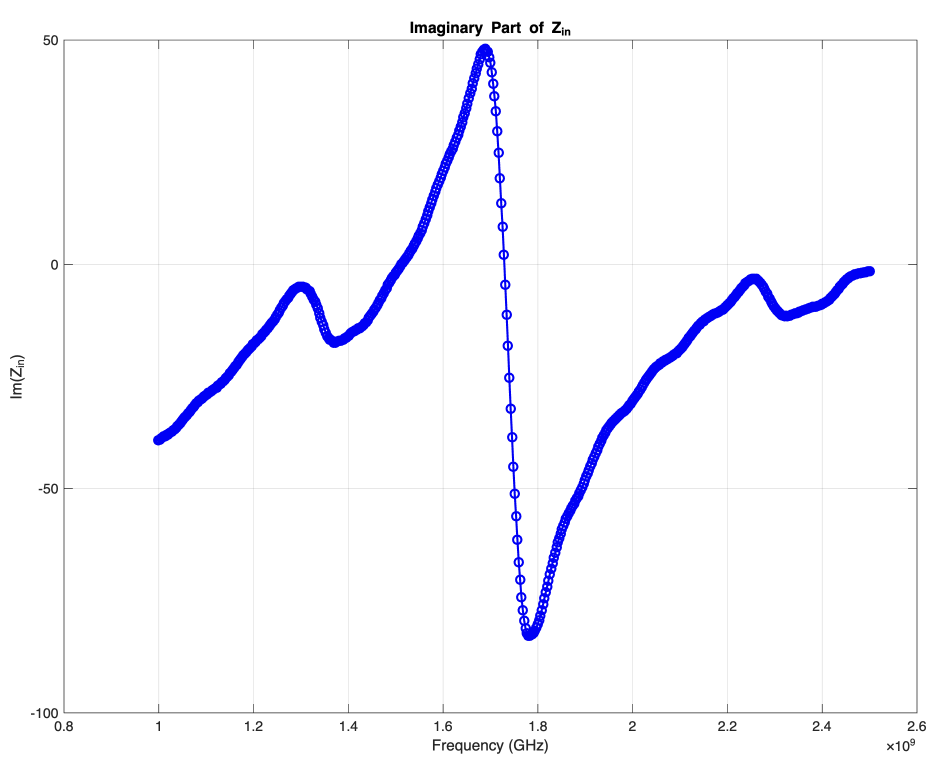
\includegraphics[width=0.5\textwidth]{./image/figure15.png}
    \caption{Imaginary Part of Input Impedance}
\end{figure}

The imaginary part of the input impedance has a similar shape to calculations from the lecture.
However, the real part is different from calculations in class. We expected it to be proportional to $\frac{1}{\sin^2(x)}$, but it only has one peak at the resonant frequency.

\subsection*{Q6}
\addcontentsline{toc}{subsection}{Q6}
See Figure 13 for the radiation plot. The results don't make sense because the minimum wave transmission occurs when the dipole antenna directly faces the reference antenna ($90 \deg$). However, we expected this to be where the maximum transmission occurs because the distance between the two antennas is the closest at that 90 $\deg$ angle. The calculation in class shows that the directivity pattern is $1.5\sin^2(\theta)$. Based on this calculation, we would expect the transmission to be more consistent across different angles because the radiation doesn't depend on which angle the dipole antenna faces.

\subsection*{Q7}
\addcontentsline{toc}{subsection}{Q7}
For step 3, $S_{21}$ is the smallest at $90 \deg$ when the dipole antenna faces the reference antenna directly. This is contrary to the belief that the maximum transmission will occur when the two antennas directly face each other. This could imply that the electric field polarization of the transmitter and receiver antenna are different.
As a result, we expect that if we rotate the dipole antenna by $90 \deg$, $S_{22}$ will be larger. However, the measured data in step 4 shows that $S_{22}$ decreased relative to that of the not rotated dipole antenna. The result deviates from the expectation because we were next to metallic objects, which reflect EM waves. Also, we carried cell phones and electronic devices near the experiment, which changed the electric field originally radiated from the dipole antenna.
\end{document}
